\documentclass[../Main.tex]{subfiles}

\begin{document}
\section{Abstract Eigenvalue Problem}
Recall from IA Vectors and Matrices that a linear map $A : V_N \mapsto V_N$ was called \underline{Hermitian} if $A^\dagger = A$, or equivalently $\langle\vec{x} ~|~(A\vec{y})\rangle = \langle(A \vec{x}) ~|~ \vec{y}\rangle$.

These had real eigenvalues, with eigenvectors corresponding to distinct eigenvalues being orthogonal. Also, these matrices were diagonalisable by choosing an orthogonal eigenvector basis.

Consider now a vector space of ``nice'' functions $f : [a, b] \mapsto \C$.\begin{definition}{Weight function}
    A \underline{weight function} $w(x) : [a, b] \mapsto \R$ is a real-valued function that is positive on $(a, b)$.
\end{definition}
Also introduce the inner product:
\begin{equation}
    \inn{f}{g}_w = \int_{a}^{b} f(x) \overline{g(x)} w(x) dx 
    \label{eqnInnerFuncProduct}
\end{equation}
And use the notation that, when $w$ is omitted, we assume $w \equiv 1$.

Let the norm be $||f||_w = \inn{f}{f}_w$.

\begin{definition}{Self-adjointness}
    A linear differential operator is \underline{self-adjoint} on $(V, \inn{\cdot}{\cdot})$ if:
    \begin{equation*}
        \inn{Ly_1}{y_2}_w = \inn{y}{Ly_2}_w
    \end{equation*}
    for all $y_1, y_2 \in V$.
\end{definition}
\begin{definition}{Eigenfunction}
    The function $y \in V \backslash \{0\}$ is an \underline{eigenfunction} for a linear differential operator $L$ if, for some $\lambda \in C$ called the \underline{eigenvalue},
    \begin{equation}
        Ly = \lambda y
        \label{eqnEigenFunc}
    \end{equation}
\end{definition}
\begin{propositions}{
        Let $L$ be self-adjoint on $V$ with respect to the inner product $\inn{\cdot}{\cdot}_w$.
        \label{propsSelfAdjProps}
    }
    \item Eigenvalues are real \label{propEValReal}
    \item Eigenfunctions with distinct eigenvalues are orthogonal with respect to the inner product \label{propEfuncOrtho}
    \item There exists a complete, orthogonal set of eigenfunctions $\{y_n\}_{n=1}^\infty$. Therefore for each $f \in V$ we can write:
        \begin{equation*}
            f = \sum_{n = 1}^\infty \hat{f}_n y_n
        \end{equation*}
        where: 
        \begin{equation*} 
            \hat{f}_n = \frac{\inn{f}{y_n}_w}{||y_n||_w^2}
        \end{equation*}
        \label{propBasisEFunctions}
\end{propositions}
\begin{proof}
    \begin{enumerate}
        \item Let $Ly = \lambda y$ for $y \neq 0$. Then:
            \begin{align*}
                (\lambda - \overline{\lambda}) ||y||_w^2 &= \inn{\lambda_y}{y}_w - \inn{y}{\lambda_y}_w \\
                &= \inn{Ly}{y}_w - \inn{y}{Ly}_w = 0
            \end{align*}
            which implies that $\lambda$ is real.
        \item If $Ly_1 = \lambda_1 y_1$, $Ly_2 = \lambda_2 y_2$,
            \begin{align*}
                &(\lambda_1 - \lambda_2) \inn{y_1}{y_2}_w \\
                &= \inn{\lambda_1 y_1}{y_2}_w - \inn{y_1}{\lambda_2 y_2} \\
                &= \inn{Ly_1}{y_2} - \inn{y_1}{Ly_2} \\
                &= 0
            \end{align*}
            which implies that $\inn{y_1}{y_2}_w = 0$.
        \item See the course II Functional Analysis.
    \end{enumerate}
\end{proof}
\section{Self-Adjoint Operators and Boundary Values}
We will study problems of the form:
\begin{align}
    Ly &= \lambda y \text{ on } x\in(a, b) \label{eqnBVProb} \\
    y &\text{ satisfies some boundary conditions} \nonumber
\end{align}
Where $L$ is a particular operator:
\begin{definition}{Sturm-Liouville operator}
    An operator $L$ is a \underline{Sturm-Liouville operator} on $(a, b)$ if it has the form:
    \begin{align*}
        Lf &= \frac{1}{w}\left[-\frac{d}{dx}\left(p \frac{d^{}f}{dx^{}}\right) + qf\right] \\
        &= \frac{1}{w}\left[-p \frac{d^{2}f}{dx^{2}} - p' \frac{d^{}f}{dx^{}} + qf\right] \\
    \end{align*}
    where $p, q, w$ are real-valued functions with $p, w > 0$ on $(a, b)$. Again $w$ is a weight function.
\end{definition}
Then we see that the eigenvalue problem $Ly = \lambda y$ is equivalent to:
\begin{equation}
    -\frac{d}{dx}\left(p \frac{dy}{dx}\right) + qy = \lambda w y
    \label{eqnSLProb}
\end{equation}
We will enforce boundary conditions in equation~\ref{eqnBVProb} by stipulating that $y$ belongs to a suitable vector space of functions that have appropriate behaviour at the boundary.
\begin{definition}{Singularity}
    For Sturm-Liouville operator on $(a, b)$, say that an endpoint $c \in \{a, b\}$ is \underline{singularity} if $p(c) = 0$.

    The opposite is non-singular, where $p(c) > 0$.
\end{definition}
We will impose real, homogeneous boundary conditions of the form:
\begin{equation}
    \alpha_c y(c) + \beta_c y'(c) = 0, \alpha_c, \beta_c \in \R, c \in \{a, b\}
    \label{eqnBoundaryCondition}
\end{equation}
where $\alpha_c$ and $\beta_c$ are not both zero, at any non-singular endpoint.

\begin{remark}
    This boundary condition is closed under addition and scalar multiplication.
\end{remark}
We will work on generic vector spaces $V \subseteq C^2[a, b]$ that require $y \in V$ to satisfy real homogeneous boundary conditions at each non-singular endpoint. We also include the inner product:
\begin{equation*}
    \inn{f}{g}_w = \int_{a}^{b} f(x) \overline{g(x)} w(x) dx 
\end{equation*}
\begin{examples}
    \item \begin{equation*}
        -\frac{d}{dx}\left[\cos\left(\frac{x}{2}\right)\frac{dy}{dx}\right] + \sin\left(\frac{x}{2}\right)y = \lambda x y
    \end{equation*}
    on $x \in (0, \pi)$, with $y'(0) = 0$. Then we have that $p(x) = \cos\left(\frac{x}{2}\right)$, $q(x) = \sin\left(\frac{x}{2}\right)$, and $w = x$. We find that $x = \pi$ is singular, so the problem is of the form $Ly = \lambda y$ with appropriate boundary conditions.
    \item \begin{equation*}
        -\frac{d}{dx}\left[(1 - x^2)\frac{dy}{dx}\right] = \lambda y, x \in (-1, 1)
    \end{equation*}
    and $p = (1 - x^2)$, $q = 0, w=1$. Therefore we do not need boundary conditions because both endpoints are singular.
\end{examples}
\begin{proposition}
    If $L$ is a Sturm-Liouville operator on $(a, b)$, with weight function $w$, then if $y_1$ and $y_2 \in C^2[a, b]$, then:
    \begin{equation}
        \inn{Ly_1}{y_2}_w - \inn{y_1}{Ly_2} = \left. p(x) W(y_1, \overline{y_2})(x)\right|_{x = a}^b
        \label{eqnSLWronskian}
    \end{equation}
    where $W(u, v)$ is the Wronskian, $W(u, v) = uv' - vu'$.
    \label{propSLWronskian}
\end{proposition}
\begin{proof}
    \begin{align*}
        \int_{a}^{b} &\frac{1}{w}\left[-(py_1')' + qy_1\right]\overline{y_2} w dx \\
        &- \int_{a}^{b} \frac{1}{w}y_1\left[ (p\overline{y_2}')' + q\overline{y_2}\right] w dx \\
        &=\int_{a}^{b} y_1 \left(p\overline{y_2}'\right)' - \overline{y_2} \left(py_1'\right)' dx 
        &= \int_{a}^{b} \frac{d}{dx}\left[p(x) W(y_1, \overline{y_2})(x)\right] dx \\
        &= \left.p(x) W(y_1, \overline{y_2})(x)\right|_{x = a}^b
    \end{align*}
\end{proof}
Now assume that $y_1, y_2$ are in a function space with appropriate boundary conditions.

If $x = c \in \{a, b\}$ is singular, then $p(c) = 0$ so the term with $x = c$ in equation~\ref{eqnSLWronskian} is zero. Alternatively, if $x = c \in \{a, b\}$ is non-singular with real homogeneous boundary conditions:
\begin{equation*}
    \begin{pmatrix}
        y_1(c) & y_1'(c) \\
        \overline{y_2}(c) & \overline{y_2}'(c)
    \end{pmatrix}
    \begin{pmatrix} \alpha_c \\ \beta_c\end{pmatrix} = \vec{0}.
\end{equation*}
And since the vector is non-zero, we must have that the determinant of the matrix, the Wronskian, is zero. That means that the term in equation~\ref{eqnSLWronskian} with $x = c$ is zero. This is all to say:
\begin{equation}
    \inn{Ly_1}{y_2} - \inn{y_1}{Ly_2} = 0
    \label{eqnSLIsSelfAdj}
\end{equation}
or, $L$ is self-adjoint.
\section{Sturm-Liouville Eigenvalue Problems}
\subsection{Solving SLEV Problems}
We now study the concrete eigenvalue problem of the form:
\begin{equation}
    -\frac{d}{dx}\left[p \frac{d^{}y}{dx^{}}\right] + qy = \lambda w y
    \label{eqnSLEvalProb}
\end{equation}
satisfying the boundary conditions in equation~\ref{eqnBoundaryCondition} at non-singular endpoints.

Then again we consider $V$ a vector space of real-valued functions in $C^2[a, b]$ satisfying the boundary conditions. Note we can assume the elements are real because $p, q, w$ are real functions, and $\lambda$ is real by proposition~\ref{propEValReal}. Then set the inner product:
\begin{equation*}
    \inn{y_1}{y_2}_W = \int_{a}^{b} y_1(x) y_2(x) w(x) dx 
\end{equation*}
Since $L$ is self-adjoint on $(V, \inn{\cdot}{\cdot})$ we apply propositions~\ref{propsSelfAdjProps} to get that there must exist $(y_n, \lambda_n) \in (V \backslash \{0\}) \times \R$ such that $Ly_n = \lambda y_n$, $\inn{y_n}{y_m} = 0$ if $\lambda_n \neq \lambda_m$, and for $f \in V$,
\begin{equation*}
    f(x) = \sum_{n=1}^{\infty}\hat{f}_n y_n(x)
\end{equation*}
where:
\begin{equation*}
    \hat{f}_n = \frac{\inn{f}{y_n}_W}{||y_n||_W^2}
\end{equation*}
are the \underline{generalised Fourier coefficients} of $f$.

It will also be the case that the $\lambda_n$ are increasing, and tend to $\infty$ as $n \to \infty$. This is proved on the example sheet.

\begin{example}
    Consider $-y'' = \lambda y$ on $0 \leq x \leq L$ with $y = 0$ at the endpoints. Then we must solve:
    \begin{equation*}
        y'' + \lambda y = 0
    \end{equation*}
    which has solution $y = A\sin(\sqrt{\lambda} x) + B\cos(\sqrt{\lambda} x)$.

    Note that if $\lambda \leq 0$ we get only trivial solutions (since the $\sin$ and $\cos$ become $\sinh$ and $\cosh$, which do not satisfy the boundary conditions). Therefore $\lambda > 0$. Applying the boundary conditions, $B = 0$ and $A\sin(\sqrt{\lambda} L) = 0$, which gives that:
    \begin{equation*}
        \lambda = \left(\frac{n\pi}{L}\right)^2
    \end{equation*}
    And therefore our $n$th solution function is:
    \begin{equation*}
        y_n(x) = \sin\left(\frac{n\pi x}{L}\right)
    \end{equation*}
    Then we can use the fact that, for $f \in V$,
    \begin{equation*}
        f(x) = \sum_{n = 1}^\infty \hat{f_n}\sin\left(\frac{n\pi x}{L}\right) 
    \end{equation*}
    where:
    \begin{align*}
        \hat{f}_n &= \frac{\inn{f}{y_n}}{||y_n||^2} \\
        &=\frac{2}{L} \int_{0}^{L} f(x) \sin\left(n\pi x\right)L dx 
    \end{align*}
    and in so doing we have re-derived the sine Fourier series!
\end{example}
\subsection{Reduction to Sturm-Liouville Form}
Consider a general eigenvalue problem of the form:
\begin{equation}
    \alpha(x) \frac{d^{2}y}{dx^{2}} + \beta(x) \frac{d^{}y}{dx^{}} + \gamma(x) y + \lambda y = 0
    \label{eqnSecondOrderEV}
\end{equation}
and constrain $\alpha(x) > 0$. Now we can use something akin to an integrating factor:
\begin{equation*}
    I(x) = \exp\left[\int^x \frac{\beta(t)}{\alpha(t)}dt\right]
\end{equation*}
\begin{proposition}
    Equation~\ref{eqnSecondOrderEV} is equivalent to:
    \begin{equation*}
        -\frac{d}{dx}\left[p \frac{dy}{dx}\right] + qy = \lambda w y
    \end{equation*}
    where:
    \begin{align*}
        p(x) &= I(x) \\
        q(x) &= \frac{-I(x) \gamma(x)}{\alpha(x)} \\
        w(x) &= \frac{I(x)}{\alpha(x)}
    \end{align*}
    \label{propEVPropEquiv}
\end{proposition}
\begin{proof}
    The proof is by dividing equation~\ref{eqnSecondOrderEV} by $\alpha$ and multiplying by $I$:
    \begin{align*}
        -\frac{d}{dx}&\left(p \frac{dy}{dx}\right) + qy - \lambda w y \\
        &= I\left[-\frac{d^{2}y}{dx^{2}} - \frac{p(x)}{\alpha(x)} \frac{d^{}y}{dx^{}}- \frac{\gamma(x)}{\alpha(x)} y - \frac{\lambda y}{\alpha(x)}\right]
    \end{align*}
    and since $I > 0$, we have that the square-bracket term must be zero whenever the Sturm-Liouville problem is zero.
\end{proof}
\begin{example}
    Consider the problem $y'' - 2y' + \lambda y = $ on $x \in [0, 1]$ with $y(0) = y'(1) = 0$.

    Then $I(x) = e^{\int^x \frac{-2}{1}} = e^{-2x}$ and so we can convert this problem to Sturm-Liouville form:
    \begin{equation*}
        -\frac{d}{dx}\left(e^{-2x} \frac{dy}{dx}\right) = \lambda e^{-2x} y
    \end{equation*}
    and note that this gives us the weight function $w(x) = e^{-2x}$.

    To solve, we substitute $y = e^{kx}$ to get $k = 1 \pm \sqrt{1 - \lambda}$. Therefore, for $\lambda \neq 1$, we have solutions of the form:
    \begin{equation*}
        y = e^x\left[Ae^{x\sqrt{1-\lambda}} + Be^{-x\sqrt{1-\lambda}}\right]
    \end{equation*}
    Then we must check that $1-\lambda < 0$ gives only trivial solutions. Then we can set $1 - \lambda = \mu^2$:
    \begin{equation*}
        y = e^x\left[A\sin(\mu x) + B\sin(\mu x)\right]
    \end{equation*}
    and so applying the boundary conditions we find $B = 0$ and $\tan{\mu} = -\mu$. By drawing the graphs of this, as shown in figure~\ref{figEValGraph} we see that there are infinitely many intersections $\mu_1, \mu_2, \cdots$.
    

    Then the eigenvalues are $\lambda_n = 1 + \mu_n^2$ with eigenfunctions $y_n = e^x \sin(\mu_n x)$. These are orthogonal with respect to the inner product:
    \begin{align*}
        \inn{y_n}{y_m} &= \int_{0}^{1} e^{-2x}y_1(x) y_2(x) dx \\
        &= \int_{0}^{1} e^{-2x} e^x \sin(\mu_n x) e^x \sin(\mu_m x) dx \\
        &= \int_{0}^{1} \sin(\mu_n x) \sin(\mu_m x) dx \\
        &= \frac12 \int_{0}^{1} \left[\cos((\mu_n - \mu_m)x) - \cos((\mu_n + \mu_m)x)\right] dx \\
        &= \frac12 \left[\frac{\sin(\mu_n - \mu_m)}{\mu_n - \mu_m} - \frac{\sin(\mu_n + \mu_m)}{\mu_n + \mu_m}\right] \\
        &= \frac12 \left[ \frac{\sin(\mu_n) \cos(\mu_m) - \sin(\mu_m \cos(\mu_n))}{\mu_n - \mu_m}\right. \\
        &\left. - \frac{\sin(\mu_n) \cos(\mu_m) + \sin(\mu_m) \cos(\mu_n)}{\mu_n + \mu_m} \right] \\
        &= \frac12 \cos(\mu_n) \cos(\mu_m) \times \left[\frac{\tan(\mu_n) - \tan(\mu_m)}{\mu_n - \mu_m} - \frac{\tan(\mu_n) + \tan(\mu_m)}{\mu_n + \mu_m}\right] \\
        &= \frac12 \cos(\mu_n) \cos(\mu_m) \left[\frac{-\mu_n + \mu_m}{\mu_n - \mu_m} - \frac{-\mu_n - \mu_m}{\mu_n + \mu_m}\right] \\
        &= \frac12 \cos(\mu_n) \cos(\mu_m) \left[-1 - (-1) \right] \\
        &=0
    \end{align*}
    although it is perfectly permissible to simply quote the result in proposition~\ref{propEfuncOrtho}.
\end{example}
\begin{figure}
    \centering
    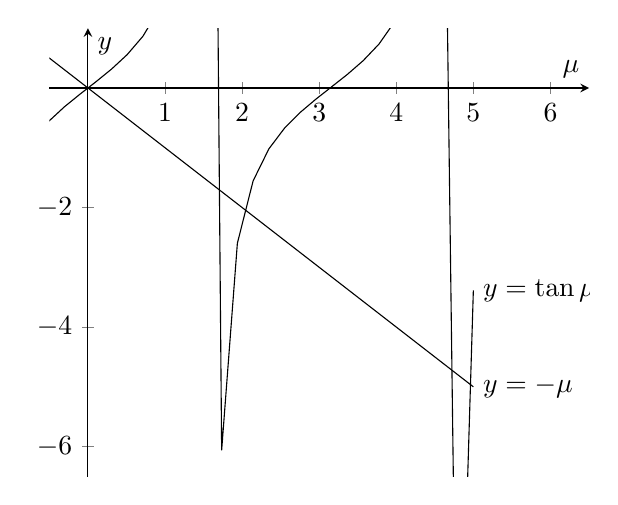
\begin{tikzpicture}[scale=1]
        \begin{axis}[
            axis lines=middle,
            xmin=-0.5,xmax=6.5,ymin=-6.5,ymax=1,
            xlabel={$\mu$},
            ylabel={$y$}
        ]
        \addplot[samples=50] {tan(deg(x))}node[right]{$y=\tan \mu$};
        \addplot[samples=50] {-x}node[right]{$y= -\mu$};
        \end{axis}
    \end{tikzpicture}
    \caption{Graph of $-\mu$ and $\tan(\mu)$}
    \label{figEValGraph}
\end{figure}
\section{Important Equations}
\subsection{Legendre's Equation}
Consider an eigenvalue problem:
\begin{equation}
    -\frac{d}{dx}\left[(1 - x)^2 \frac{dy}{dx}\right] = \lambda y, x \in (-1, 1)
    \label{eqnLegendre}
\end{equation}
Then we find that $p = (1 - x^2), q = 0, w = 1$. Then we note that both endpoints are singular, so as we have seen we do not have to specify boundary conditions. Therefore, we consider only the space $V = C^2[-1, 1]$.

Since $x = 0$ is a regular singular point of the differential equation, we can look for solutions of the form:
\begin{equation*}
    y = \sum_{n=0}^{\infty} a_n x^n
\end{equation*}
then from IA Differential Equations, we can find a recurrence relation for the $a_n$ that depend on $a_0$ and $a_1$:
\begin{equation*}
    a_{n+2} = \left[\frac{n(n+1)-\lambda}{(n+1)(n+2)}\right]a_n
\end{equation*}
This gives us two linearly independent solutions, depending on the parity of the terms:
\begin{align*}
    y_0(x) &= a_0 \left[1 + \frac{-\lambda x^2}{2!} + \frac{-\lambda (6-\lambda)x^4}{4!} + \cdots\right] \\
    y_1(x) &= a_1 \left[x + \frac{(2-\lambda)x^3}{3!} + \frac{(2-\lambda)(12-\lambda)x^5}{5!} + \cdots\right]
\end{align*}
note that one of the equations collapses (terminates) to give a polynomial if, for some $k \in \N \cup \{0\}$, $\lambda = k(k+1)$.

If $\lambda$ does not have this form, we have two infinite series. We note that $\frac{a_{n+2}}{a_n} \to 1$ as $n \to \infty$, so we must have that both series will converge on $|x| < 1$. However, we need convergence on also $|x| = 1$ for the solution to be valid.

\begin{proof}[Non-examinable proof that $y_0$ diverges at $|x| = 1$]
    Let $A_n = a_{2n}$, so:
    \begin{equation*}
        \frac{A_n}{A_{n+1}} = \frac{(2n+1)(2n+2)}{2n(2n+1) - \lambda} = 1 + \frac{1}{n} + \epsilon_n
    \end{equation*}
    where $|\epsilon_n| \leq \frac{M}{n^2}$ where $M$ is a positive constant (that depends on $\lambda$). That is, the RHS is positive for $n$ sufficiently large. Say that this is the case when $n \geq N$, $N \in \N$. In particular, the $A_n$ must all have the same sign when $n \geq N$.
    We then want to find some bounds. Note that we can use $e^x \geq 1 + x$:
    \begin{align*}
        \frac{|A_n|}{|A_{n+1}|} &\leq e^\frac1{n} + \epsilon_n \\
        \implies |A_{n+1}| & \geq \frac{e^{-\frac{1}{n}}|A_n|}{1 + e^{-\frac{1}{n}}|\epsilon_n|} \\
        &\geq \frac{e^{-\frac{1}{n}}|A_n|}{1 + |\epsilon_n|} \\
        &\geq e^{-\frac{1}{n}} |A_n|e^{-|\epsilon_n} \\
    \end{align*}
    and by repeating this, for $n \geq N$,
    \begin{align*}
        |A_{n+1}| &\geq |a_n| \exp\left[-\left(\frac{1}{n} + \frac{1}{n-1} + \cdots + \frac{1}{N}\right)\right. \\
        &- \left.\left(|\epsilon_n| + \cdots + |\epsilon_N|\right)\right] \\
    \end{align*}
    Then defining the harmonic series $H_n = \sum_{i=1}^{n} \frac{1}{i}$,
    \begin{equation*}
        |A_{n+1} \geq |A_n| e^{-H_n + H_{N-1}} e^{-M\frac{\pi^2}{6}}
    \end{equation*}
    Because the sum of $\epsilon_n$ is:
    \begin{align*}
        |\epsilon_n| &+ \cdots + |\epsilon_N| \\
        &\leq M\left[\frac{1}{n^2} + \cdots + \frac{1}{N^2}\right] \\
        &\leq M\sum_{k=1}^\infty \frac{1}{k^2} \\
        &= \frac{M\pi^2}{6}
    \end{align*}
    Now since $H_n \leq \log(n) + 2\gamma$,
    \begin{align*}
        |A_{n+1}| &\geq |A_N| e^{H_{N-1} = M\frac{\pi^2}{6}} e^{-\log(n) - 2\gamma} \\
        &> \frac{C}{n+1}
    \end{align*}       
    Then $y_0$ is given by:
    \begin{equation*}
        y_0 = \sum_{n \leq N} A_n x^{2n} + \sum_{n > N} A_nx^{2n}
    \end{equation*}
    then since the $A_n$ have the same sign, we assume they are positive WLOG.
    \begin{align*}
        \sum_{n > n} A_n x^{2n} &> c\left[\sum_{n=1}^\infty \frac{x^{2n}}{n} - \sum_{n \leq N}  \frac{x^{2n}}{n}\right] \\
        &= c\left[\log\left(\frac{1}{1-x^2}\right) - \text{polynomial in x}\right]
    \end{align*}
    and by considering the $\log$ term, we see that this diverges at $x = \pm 1$.

    The analysis is similar for $y_1$
\end{proof}
Thus if the functions $y_0$ or $y_1$ does not collapse into a polynomial, it is not in $V$. Therefore, the solutions to Legendre's equation (\ref{eqnLegendre}) are the ``Legendre polynomials'' where $\lambda = k(k+1)$. We often make a normalisation $y(1) = 1$.

\begin{tabular}{|c|c|c|}
    \hline
    $k$ & $\lambda_k$ & $p_k(x)$ \\
    \hline
    $0$ & $0$ & $p_0(x) = 1$ \\
    $1$ & $2$ & $p_1(x) = x$ \\
    $2$ & $6$ & $p_2(x) = \frac12(3x^2-1)$ \\
    $3$ & $12$ & $p_1(x) = \frac12(5x^3-3x)$ \\
    \hline
\end{tabular}
\subsection{Bessel's Equation}
Fix an integer $m \geq 0$. Consider:
\begin{equation}
    -\frac{d}{dr} \left[r \frac{dy}{dx}\right] + \frac{m^2}{r}y = \lambda r y, r \in (0, 1), y(1) = 0
    \label{eqnBesselSL}
\end{equation}
Here we have $p = r, q = \frac{m^2}{r}, w = r$. We have that the left endpoint is singular so we only need the 1 boundary condition.

We can change this into standard form:
\begin{equation}
    r^2 y'' + ry' + \left(\lambda r^2 - m^2\right)y = 0, r\in(0, 1), y(1) = 0
    \label{eqnBesselStd}
\end{equation}
Then we can set $z = \sqrt{\lambda} r$. Note that here $\lambda$ is unknown but we can show it is non-negative. Also set $R(z) = y(r)$.
\begin{equation}
    z^2 R'' + zR' + (z^2 - m^2)R = 0, z \in (0, \sqrt{\lambda}), R(\sqrt{\lambda}) = 0
    \label{eqnBessel}
\end{equation}
and this is Bessel's Equation. By substituting in the form:
\begin{equation*}
    R = z^\sigma \sum_{n=0}^{\infty} a_n z^n
\end{equation*}
we get two linearly independent solutions. Without going into detail, only 1 solution is well-behaved at 0, $J_m(z)$:
\begin{equation}
    J_m(z) = \left(\frac{z}{2}\right)^m \sum_{n=0}^{\infty} \frac{(-1)^n}{n!(n+m)!} \left(\frac{z}{2}\right)^{2n}
    \label{eqnBesselSoln}
\end{equation}
These are called \underline{Bessel's Functions of the First Kind} (the second kind is the set of solutions that are badly behaved at 0).
Also, we can show that as $z \to \infty$,
\begin{equation*}
    J_m(z) \to \sqrt{\frac{2}{\pi z}} \cos\left(z - \frac{\pi m}{2} - \frac{\pi}{4}\right) + O(z^{-\frac{3}{2}})
\end{equation*}
so $J_m(z)$ has infinitely many zeroes on the positive $z$-axis, labelled $j_{mk}$ for $k \in \N$. Since we require that $J_m(\sqrt{\lambda}) = 0$, we have the eigenvalues $\lambda_k = j_{mk}^2$. That is, solutions to equation~\ref{eqnBesselSL} are:
\begin{equation}
    y_k(r) = J_m(j_{mk}r), \lambda_k = j_{mk}^2
    \label{eqnBesselSLSoln}
\end{equation}
\subsection{Inhomogeneous Problems}
Let $L$ be a Sturm-Liouville operator. Consider problems of the form:
\begin{equation*}
    Ly = f \in V
\end{equation*}
After possibly re-labelling the function $f$, set $w = 1$. Because $L$ is Sturm-Liouville, we have $\{Y_k\}$ a set of normalised eigenfunctions of $L$, and by completeness we can write, for any $y \in V$:
\begin{equation*}
    y = \sum_{k} A_k Y_k,~~f = \sum_k B_k Y_k
\end{equation*}
which gives:
\begin{align*}
    \sum_{j=1}^{\infty} (\lambda_k A_k - B_k) Y_k &= 0 \\
    \implies \lambda_k A_k &= B_k \\
    \implies A_k \frac{B_k}{\lambda_k} \text{ if all } \lambda_k \text{ are non-zero}
\end{align*}
which gives our solution:
\begin{equation*}
    y(x) = \sum_{k=1}^{\infty} \frac{B_k}{\lambda_k} Y_k(x)
\end{equation*}
where $B_k = \inn{f}{Y_k}$. Applying this:
\begin{align*}
    y(x) &= \sum_{j=1}^{\infty} \frac{1}{\lambda_k} \left[\int_{a}^{b} f(\xi) Y_k(\xi) d\xi \right]Y_k(x)
    &= \int_{a}^{b} G(x;\xi) f(\xi) d\xi 
\end{align*}
Where
\begin{equation*}
    G(x;\xi) = \sum_{k=1}^{\infty} \frac{Y_k(\xi)Y_k(x)}{\lambda_k}
\end{equation*}
Here $G$ is a Green's Function.
\end{document}